% ============================================================
%  CRD - IEEE ICME 2027 submission draft
%  Template : IEEEtran conference class (generic IEEE conference template)
%  Build    : pdflatex -> bibtex -> pdflatex x2   (see README.md)
%
%  NOTE  ICME 2027 has not yet published its own LaTeX kit or page limit.
%        This file uses the generic IEEE conference template only.
%        Author block / anonymity / copyright are placeholders.
% ============================================================
\documentclass[conference]{IEEEtran}

\usepackage{amsmath}
\usepackage{amssymb}
\usepackage{graphicx}
\usepackage{booktabs}
\usepackage{needspace}
\usepackage{url}
\usepackage[hidelinks]{hyperref}

\graphicspath{{fig/}}
\setlength{\textfloatsep}{2pt plus 1pt minus 1pt}
\setlength{\floatsep}{2pt plus 1pt minus 1pt}
\setlength{\intextsep}{2pt plus 1pt minus 1pt}

\begin{document}

\title{CRD: Cross-Modal Residual Debiasing for\\
Global Noisy Image--Text Pair Detection}

% TODO: replace with the real author block once ICME 2027 publishes the
% author / anonymity / copyright requirements.
\author{\IEEEauthorblockN{Anonymous Submission}
\IEEEauthorblockA{Paper ID 0000}}

\maketitle

% ============================================================
%  Abstract
% ============================================================
\begin{abstract}
Curating web-scale image--text data usually amounts to thresholding a frozen
vision--language similarity, which presupposes that scores are comparable across
pairs. On the Attribute facet of a controlled benchmark, raw CLIP similarity orders
$31.9\%$ of all clean/noisy pair combinations backwards, although the same encoder
separates the two classes far above chance. We attribute part of this behaviour to
additive score components that are predictable from the image and text features and
largely unrelated to whether a pair matches. CRD (cross-modal residual debiasing),
a post-hoc calibration, fits two small additive heads on the frozen features and
subtracts a scaled estimate of the component from the standardised similarity; inference needs
one pair, no reference bank, and labels only to select one scalar. We also present
FGBench, $88{,}024$ reciprocal cycles over five factual facets from COCO and Visual
Genome, with silver labels. On the three reported Attribute backbones CRD raises
AUROC (CLIP ViT-B/16: $0.6806\to0.7187$; SigLIP2: $0.7026\to0.7509$); $21$ of $24$
paired comparisons survive Holm, or $17$ of $20$ independent comparisons once four
monotone GMM duplicates are excluded. Two parameter-free debiasing baselines do not
reproduce the Attribute gain. A logistic-regression probe trained on a
$32{,}000$-row labeled subset is $0.47$ and $1.60$ points higher on Attribute and
Quantity, and an MLP probe $7.62$ higher on the exploratory Action facet, at the cost
of about four times CRD's label budget; at CRD's budget the logistic-regression probe
falls $4.36$ points below CRD on Attribute. The method leaves cycle-level forced-choice
accuracy (2AFC) unchanged by construction and does not surpass CSLS on Quantity or
Entity.
\end{abstract}


\begin{IEEEkeywords}
noisy image--text pairs, cross-modal similarity, score calibration,
vision--language models, data curation, benchmark
\end{IEEEkeywords}

\begin{figure*}[!t]
  \centering
  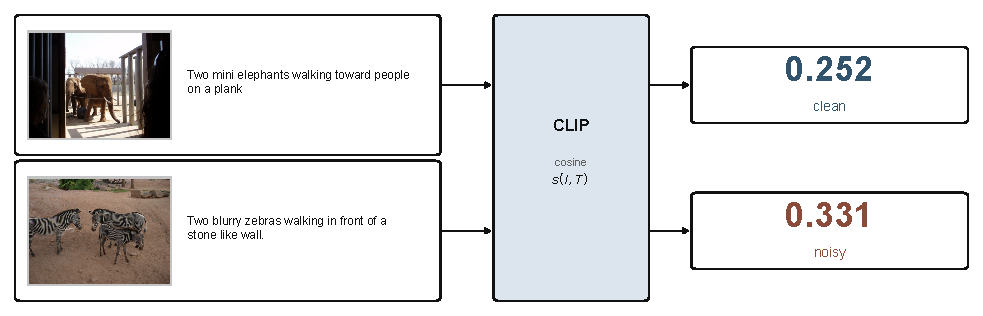
\includegraphics[width=0.94\textwidth]{fig1_coco.pdf}
  \caption{Raw image--text similarity does not rank a correct pair above an
  incorrect one. Both pairs come from the COCO Quantity facet and are scored by
  the same frozen CLIP ViT-B/16; neither score was modified. The correctly
  matched pair (top) scores $0.252$, while the pair whose caption states the
  wrong number of animals (bottom) scores $0.331$. A threshold on the raw score
  therefore separates the two in the wrong direction. Images are the original
  COCO images.}
  \label{fig:motivation}
\end{figure*}

% ============================================================
%  Introduction
% ============================================================
\section{Introduction}
\label{sec:intro}

Vision--language models~\cite{radford2021clip,li2022blip} are now the standard
instrument for assembling image--text corpora: a candidate pool is encoded, every
pair receives a similarity, and pairs below a threshold are discarded or queued for
relabelling. This presumes that a similarity can be compared \emph{across} pairs,
that a pair scoring $0.33$ is noisier than one scoring $0.25$. The premise fails.
Figure~\ref{fig:motivation} shows a correctly matched pair scoring $0.252$ and a
pair whose caption misstates the number of animals scoring $0.331$ under the same
frozen encoder.

Existing detectors intervene on the encoder or on the neighbourhood. CSLS
re-normalises a score against a neighbour set, matching heads replace it with a
learned score, and LEMoN judges a pair by its agreement with multimodal neighbours,
while TRACED edits the caption and reads the resulting similarity trajectory. Each improves the signal that is subsequently
thresholded, and each leaves one question unanswered: for a fixed signal, do two
unrelated pairs share a scale? Capacity does not settle it within the zero-shot CLIP
family: ViT-L/14, with $427.6$M parameters against $149.6$M, leaves Attribute AUROC
at $0.6779$ against $0.6806$. The deficiency is not the representation but the
absence of an explicit model of the score component that should not enter a global
comparison.

We therefore model the additively predictable part of the standardised similarity
as $g_\theta=a_\phi(u)+b_\psi(v)+b_0$, fit it to each pair's own score without using
a label, and subtract it at inference, $z'=z-\lambda g_\theta$. The
encoder is frozen; inference consumes one pair, with no reference bank, partner
caption or cycle; labels enter only the selection of $\lambda$. We evaluate on
FGBench, $88{,}024$ reciprocal cycles over five factual facets derived from COCO and
Visual Genome.

\needspace{5\baselineskip}
\noindent\textbf{Contributions.}
\begin{itemize}
  \item \textbf{Method.} CRD, a post-hoc calibration that estimates additive
  image- and text-conditioned score components with two lightweight heads over a
  frozen encoder and subtracts them from the standardised similarity, improving
  global discrimination without any reference structure at inference.
  \item \textbf{Benchmark.} FGBench, an $88{,}024$-cycle reciprocal benchmark with
  five factual facets, explicit split hygiene and an automatic split/leakage audit.
  \item \textbf{Analysis.} Paired tests against five same-backbone detectors and two
  parameter-free debiasing baselines, ablations, selected frozen backbones, and an
  explicit account of where the calibration stops helping.
\end{itemize}

% ============================================================
%  Related Work
% ============================================================
\section{Related Work}
\label{sec:related}

Noise detection on frozen contrastive encoders~\cite{radford2021clip,li2022blip,zhai2023siglip}
has proceeded along three lines. The first rescales the score: hubness-corrected
variants such as CSLS~\cite{conneau2018csls} re-normalise each score against a
neighbour set, and density models threshold an estimated noise rate. The second
replaces the score with a learned matcher, typically an image--text matching head.
The third exploits relational structure: LEMoN~\cite{zhang2024lemon} judges a pair
by its agreement with multimodal neighbours, and TRACED~\cite{afriat2025traced}
edits the caption and reads the resulting similarity trajectory. The latter two are
effective but presuppose a reference bank, a batch of other pairs, or an editing
model; the present setting is one pair in and one score out, with no other sample.

Score incomparability is documented in retrieval; remedies re-normalise against a
reference set, apply a monotone transform, or fit a distribution. CRD is additive like
CSLS, but its correction is regressed on the pair's own score and needs no bank. A
monotone transform leaves ranking unchanged (GMM, Table~\ref{tab:main});
compositionality benchmarks such as FOIL~\cite{shekhar2017foil} and
SugarCrepe~\cite{hsieh2023sugarcrepe} compare two captions for one image, so
per-image offsets cancel.

% ============================================================
%  Problem Formulation and Motivation
% ============================================================
\section{Problem and Method}
\label{sec:problem}

\subsection{Task Definition}
Let $f_I$ and $f_T$ be frozen image and text encoders and $u=f_I(I)$, $v=f_T(T)$.
The raw score is the cosine similarity $s(I,T)=\operatorname{sim}(u,v)$, and each
pair carries a binary label $y\in\{0,1\}$ (clean or noisy). The task is to construct
$q(I,T)$ whose ranking separates the classes better than $s$. Two properties
distinguish it from same-image candidate ranking: the comparison is \emph{global}
(the two pairs share neither image nor caption) and scoring is \emph{pair-local}
($q$ may not depend on which other pairs are present). We therefore report cross-pair
AUROC and cycle-level 2AFC (two-alternative forced choice) separately.

\subsection{Empirical Limitation of Raw Similarity}
Figure~\ref{fig:motivation} shows a COCO Quantity example scored by one frozen CLIP
ViT-B/16: the correct pair scores $0.252$, the pair whose caption misstates the
number of animals $0.331$. A single case proves little, so we quantify it on the
largest facet where the effect is measurable, Visual Genome Attribute. Comparing every clean
pair with every noisy pair, $31.9\%$ of the comparisons place the noisy pair above
the clean one, which equals $1-\mathrm{AUROC}$ ($1-0.6806$); the corresponding value
for Quantity is $16.9\%$ ($1-0.8305$). Within one reciprocal cycle, replacing the
caption of a fixed image changes the score ($0.324\to0.188$) and replacing the image
changes it too ($0.324\to0.253$), so the score depends on which image and caption are
involved, not solely on whether they correspond. These are conditioned variations,
not measurements of an isolated modality bias.

\subsection{Hypothesis: Additive Score Components}
Suppose the standardised score decomposes as
\begin{equation}
  z \;=\; \underbrace{m(I,T)}_{\text{cross-modal match}} \;+\;
         \underbrace{c(I,T)}_{\text{additive component}},
  \label{eq:decomp}
\end{equation}
where $c$ is predictable from $u$ and $v$ and largely independent of whether they
correspond. Under \eqref{eq:decomp}, a stronger encoder raises the first term while
the ordering of unrelated pairs remains governed by the second, consistent with the
unchanged Attribute AUROC of ViT-L/14. The decomposition also explains why a monotone
recalibration cannot help: it acts on $z$ as a whole. Equation~\eqref{eq:decomp} is a
modelling assumption, not a generative account, and we do not claim that $c$ is
identifiable as image or text noise. What is tested is its operative consequence: if
a component of $z$ is predictable from $u$ and $v$ alone, removing that prediction
should improve global discrimination, and a control fitted to permuted targets
should not.

\begin{figure*}[!t]
  \centering
  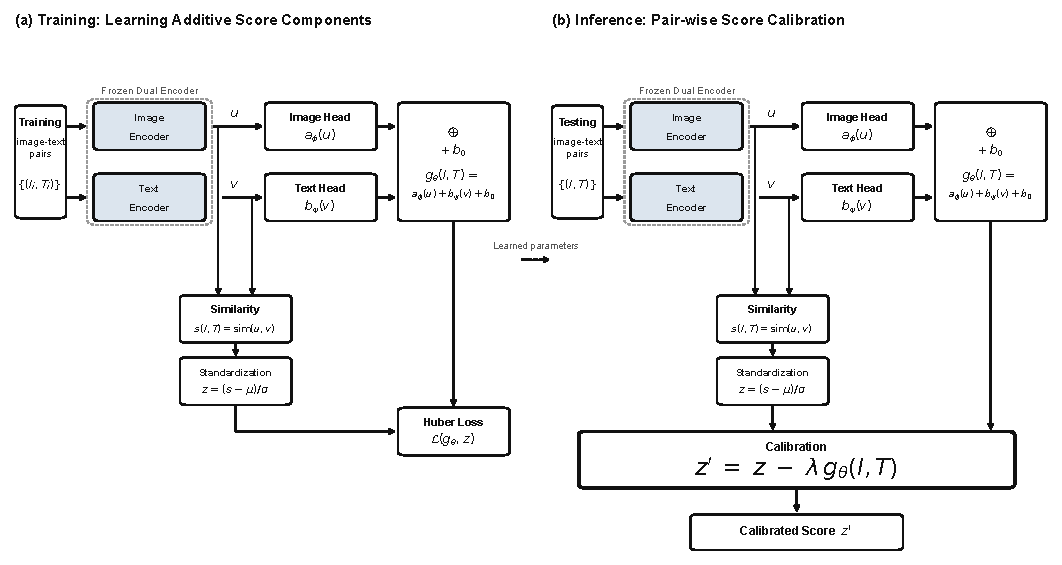
\includegraphics[width=0.88\textwidth]{fig2_crd.pdf}
  \caption{Overview of the proposed CRD framework. (a) During training, CRD
  learns additive image-conditioned and text-conditioned score components from
  row-level standardised image--text similarity scores. Both encoders are frozen
  and only the two heads and the bias $b_0$ are optimised. (b) During inference,
  the estimated additive component is subtracted from the raw standardised
  similarity to obtain a calibrated pair-wise score. The heads and the statistics
  $\mu,\sigma$ are fixed from training and $\lambda$ is chosen on a validation
  split; a single pair is sufficient and no reference bank or cycle is used.}
  \label{fig:overview}
\end{figure*}

% ============================================================
%  Method: Cross-modal Score Calibration (CRD)
% ============================================================
\subsection{CRD Overview}
\label{sec:method}
CRD is a post-hoc calibration layer. It modifies neither encoder, adds two small
heads, and returns a corrected score for a single pair. Figure~\ref{fig:overview}
shows the path: the pair is encoded, the additive heads are regressed onto the
standardised similarity, and inference combines the raw score with one subtraction.
No encoder parameter is updated, and inference never observes a label.

\subsection{Frozen Features and Score Standardisation}
For a pair $(I,T)$ we compute
\begin{equation}
  u = f_I(I), \qquad v = f_T(T), \qquad s(I,T) = \operatorname{sim}(u,v),
\end{equation}
with $\operatorname{sim}$ the cosine similarity. Because similarity scales differ
between encoders, the score is standardised with statistics estimated on the
training split alone,
\begin{equation}
  \mu = \operatorname*{mean}_{\mathcal{D}_{\text{train}}} s, \qquad
  \sigma = \operatorname*{std}_{\mathcal{D}_{\text{train}}} s + 10^{-8}, \qquad
  z = \frac{s-\mu}{\sigma}.
  \label{eq:z}
\end{equation}
Validation and test pairs use the same $\mu,\sigma$; no statistic is computed on
either split. Standardisation makes one $\lambda$ grid meaningful across backbones
with different ranges and places the target on the scale of the residual.

\subsection{Additive Score Estimation}
The estimated component is a sum of two head outputs and a bias,
\begin{equation}
  g_\theta(I,T) \;=\; a_\phi(u) + b_\psi(v) + b_0,
  \label{eq:g}
\end{equation}
where each head is a two-layer perceptron with one hidden layer of width $64$ and a
GELU nonlinearity. The additive form is retained in preference to a joint residual
network over concatenated features: a joint network can absorb part of the match term
$m(I,T)$, so the constraint is a design choice rather than a mathematical necessity. Here $g_\theta$ is neither a second similarity nor an estimate of image or text
noise; it is the component of $z$ predictable from the two sides jointly, with no
cross-side interaction term.

\subsection{Row-level Objective and Inference}
Each training pair contributes one target, its own standardised score $z$:
\begin{equation}
  \mathcal{L}(\theta) = \frac{1}{|\mathcal{D}_{\text{train}}|}
  \sum_{(I,T)} \operatorname{Huber}\!\left(g_\theta(I,T),\, z(I,T)\right).
  \label{eq:loss}
\end{equation}
Supervising on the pair's own score, rather than on its cycle mean, is substantive:
the matched and mismatched members of a cycle share the same cycle mean, so a
cycle-mean target asks the heads to predict a quantity that is constant within the
group being ranked. The encoders are frozen and only $\phi,\psi,b_0$ are optimised;
the regression target involves no clean/noisy label. Labels enter at exactly one
point, the selection of $\lambda$; the method is therefore not fully unsupervised and
is not described as such.

The calibrated score is
\begin{equation}
  z' \;=\; z \;-\; \lambda\, g_\theta(I,T),
  \label{eq:calib}
\end{equation}
with $\lambda\ge0$ selected on a validation split (for Attribute, $2{,}084$ cycles)
by maximising the AUROC of $z'$, over $\Lambda=\{0,0.1,\dots,2.0\}$. The grid
includes zero, so validation can decide that no calibration is warranted; in the
placebo runs it does. Selected values are not restricted to $[0,1]$ (they range from
$0.8$ to $1.4$ across our cells), so the operation is a scaled subtraction rather
than an exact removal. Inference is pair-local: the features are encoded once, the two heads
are evaluated, and \eqref{eq:calib} is returned, with no reference bank, partner
caption or test-time threshold. The heads hold $65{,}795$ parameters and cost
$0.2$\,ms; end to end the calibrated score adds $0.83$\,ms ($5.5\%$) to a
$15.1$\,ms CLIP ViT-B/16 pass. Training details are given in Section~\ref{sec:exp}.

% ============================================================
%  FGBench
% ============================================================
\section{FGBench: Benchmark Construction}
\label{sec:fgbench}

FGBench asks which of two unrelated pairs is noisier, and its construction follows
from that question. Every image and caption is an existing COCO~\cite{lin2014coco} or
Visual Genome~\cite{krishna2017vg} item; a mismatch is produced by contradicting a
structured fact attached to the image, so the label rests on an external
justification. Splits are disjoint at the cycle level, and the construction is
auditable.

For an image pair $(A,B)$ with captions $(T_A,T_B)$ we emit four records
\begin{equation}
\begin{aligned}
  &(A,T_A,\text{clean}),\quad (B,T_A,\text{noisy}),\\
  &(B,T_B,\text{clean}),\quad (A,T_B,\text{noisy}),
\end{aligned}
\end{equation}
a reciprocal cycle. Each image and caption occurs once as a match and once as a
mismatch, so every facet is exactly $50\%$ balanced and the two classes share the
same distributions over image and text sides. A detector cannot exploit the frequency
of an image or caption to separate the classes. The cycle is a property of the data,
not of the method: CRD is trained on individual pairs and scores one pair at
inference.

Five facets come from two sources. From COCO we build \textbf{Entity} (object
category substituted) and \textbf{Quantity} (numeral substituted); from Visual Genome
we build \textbf{Attribute} (colour, material or state), \textbf{Action} (predicate)
and \textbf{Relation} (spatial or comparative relation), all from VG150-style
annotations.

\begin{table}[t]
\centering
\small
\setlength{\tabcolsep}{4pt}
\caption{FGBench v1-strict. Every cycle contributes two matched and two mismatched
pairs, so each facet is exactly balanced. The test split, used by all methods,
contains $17{,}565$ cycles and $70{,}260$ pairs; per-facet test sizes make the
statistical power of each column explicit.}
\label{tab:fgbench}
\begin{tabular}{llrrr}
\toprule
Source & Facet & Cycles & Pairs & Test (cycles) \\
\midrule
COCO          & Entity     & 32{,}589 & 130{,}356 &  2{,}298 \\
COCO          & Quantity   &  2{,}940 &  11{,}760 &    114 \\
Visual Genome & Attribute  & 49{,}042 & 196{,}168 & 14{,}281 \\
Visual Genome & Action     &    567   &   2{,}268 &    166 \\
Visual Genome & Relation   &  2{,}886 &  11{,}544 &    706 \\
\midrule
\multicolumn{2}{l}{Total}      & 88{,}024 & 352{,}096 & 17{,}565 \\
\bottomrule
\end{tabular}
\end{table}

Table~\ref{tab:fgbench} summarizes the construction. Labels are \emph{silver}: they
follow from a substitution rule applied to a structured annotation, not from human
adjudication. An annotation records what was
annotated, not a complete inventory of the image, so unannotated content is treated
as unknown rather than absent; a strict tier retains only Relation cases with
unambiguous annotation support and removes $276$ cycles ($1{,}104$ rows) whose labels
rely on six ambiguous rules; all numbers here refer to v1-strict. All detectors are
evaluated on the identical manifest. The benchmark audit reports a maximum of one
split per image and per caption and evidence completeness $1.000$. Because every
image and caption occurs once in each class, any single-side score has identical
class-conditional distributions; the TF-IDF check is therefore an analytic invariant
($0.5000$), not independent evidence, and the construction makes a text-only shortcut
impossible by design.

% ============================================================
%  Experiments
% ============================================================
\section{Experiments}
\label{sec:exp}

\subsection{Experimental Setup}
All methods share one frozen CLIP ViT-B/16 encoder unless stated, so rows of
Table~\ref{tab:main} differ in post-processing and auxiliary inputs, not in the
representation; Section~\ref{sec:cross} repeats the comparison on two further frozen
encoders (ViT-L/14 and SigLIP2). Heads are optimised with AdamW for $1{,}500$ iterations at batch size
$256$, learning rate $10^{-3}$, weight decay $10^{-4}$ and the Huber loss with its
default transition; three seeds share a fixed training subset, row order and therefore
$\mu,\sigma$, and hashes of the manifest, feature cache and row order are verified to
agree. The primary metric is AUROC over pairs; AUPRC is secondary; 2AFC is reported
separately because it is not interchangeable with AUROC. Values are mean $\pm$
standard deviation over three seeds; the data subset is fixed. Comparisons use a cycle-clustered paired
bootstrap with Holm correction over the $24$ cells;
CSLS's $\lambda$ is selected on the same validation split; re-selecting it on a
$0$--$30$ grid leaves the Quantity/Entity ordering unchanged. The Action facet's
official validation split contains two cycles, so for that facet only $20\%$ of the
training cycles ($80$ of $399$) are held out, with no image shared with the retained
cycles; this is a single fixed draw and a protocol deviation. Its $166$ test cycles
are untouched, and the Action cells are marked $\dagger$ and treated as exploratory.

\subsection{Comparison with Same-Backbone Detectors}
Table~\ref{tab:main} compares CRD with a cosine threshold, CSLS, a GMM density
detector, LEMoN-style and TRACED-style reproductions, two parameter-free
feature-debiasing baselines (mean-centred and all-but-the-top (ABTT) cosine), and a
supervised probe used as a reference ceiling. The
two debiasing baselines are the null hypothesis: they ask whether the gain comes from
the learned heads or merely from removing first-order feature structure. Both are
fitted on the training split only, with no gradient training; the single
hyper-parameter ($k$ for ABTT) is selected on the same validation split as $\lambda$.
LEMoN uses the official adapter on the same cached CLIP features and test split:
IndexFlatIP neighbour retrieval with $k{=}5$, the official
$d_1+\beta d_n+\gamma d_m$ score, and hyperparameters fitted on the validation split.
TRACED is a mechanism-level reproduction: it builds a deletion-only caption trajectory
of three steps; because its token-replacement operator is not reproduced, it is treated
as a lower bound.

\begin{table*}[t]
\centering
\footnotesize
\setlength{\tabcolsep}{9pt}
\caption{AUROC on FGBench v1-strict, frozen CLIP ViT-B/16. CRD is mean $\pm$ std over
seeds; baselines are single-run. $^\dagger$Action uses an internal validation split.
GMM/mean-centred/ABTT are controls; the LR probe is reported in the text. The Holm
family is five method rows $\times$ five facets minus GMM/Action ($24$ cells; four
GMM duplicates leave $20$ independent).}
\label{tab:main}
\begin{tabular}{lccccc}
\toprule
Method & Entity & Quantity & Attribute & Action$^\dagger$ & Relation \\
\midrule
CLIP cosine                & 0.9991 & 0.8305 & 0.6806 & 0.5913 & 0.5413 \\
CLIP + CSLS                & \textbf{0.9996} & 0.8882 & 0.6866 & 0.5869 & 0.5417 \\
LEMoN (official)           & 0.9990 & 0.8266 & 0.6755 & 0.5923 & 0.5218 \\
TRACED-style               & 0.9985 & 0.8412 & 0.6875 & 0.6102 & 0.5356 \\
\midrule
\multicolumn{6}{l}{\emph{Controls (not detectors)}}\\
GMM (monotone)             & 0.9991 & 0.8305 & 0.6806 & --- & 0.5413 \\
Mean-centred cosine        & 0.9989 & 0.8570 & 0.6790 & 0.5890 & 0.5389 \\
ABTT cosine                & 0.9985 & 0.8481 & 0.6765 & 0.5394 & 0.5464 \\
\midrule
\textbf{CRD (ours)}        & \shortstack{0.9995\\\scriptsize$\pm$0.0000} & \shortstack{0.8837\\\scriptsize$\pm$0.0011} & \shortstack{0.7187\\\scriptsize$\pm$0.0001} & \shortstack{0.6145\\\scriptsize$\pm$0.0009} & \shortstack{\textbf{0.5530}\\\scriptsize$\pm$0.0001} \\
\bottomrule
\end{tabular}
\end{table*}

On Attribute, CRD improves AUROC by $3.81$ points on the seed mean (arithmetic
difference; the bootstrap mean is $3.84$) and by $3.12$ to $4.32$ points over the
five detector/control rows in Table~\ref{tab:main} (cosine, CSLS, GMM, LEMoN official
and TRACED-style), with a 95\% CI of $[3.73,3.96]$ against cosine. The absolute gain is larger on Quantity ($+5.32$), but CSLS already
accounts for most of it. On Action CRD reaches $0.6145$ against $0.6102$ for TRACED,
a paired-bootstrap difference of $+0.43$\,pp (95\% CI $[-1.75,2.54]$), which does
not survive Holm; we claim parity rather than superiority. On Quantity and Entity the ordering reverses
on the seed-mean convention (CSLS $0.8882$ against $0.8837$; $0.9996$ against
$0.9995$; seed-mean Entity scores are tied), so CRD is not described as uniformly
better. Across the $24$ cells, $21$ are significant after Holm; four of these are the
monotone GMM control, whose AUROC is identical to cosine by construction, so the
independent count is $17$ of $20$. The exceptions are Entity against CSLS, Quantity
against CSLS and Action against TRACED. The Entity gain
over cosine, although significant, is $0.04$ points where every method exceeds
$0.9985$ and is not read as a practical gain.

The comparison against the debiasing baselines is consistent. As a separate family of
ten tests, CRD is better than mean-centred cosine, on the seed-mean score, by
$3.97$ (Attribute), $2.67$ (Quantity), $2.55$ (Action), $1.41$ (Relation) and $0.06$
(Entity) pp, and better than ABTT by $4.22$, $3.56$, $7.51$, $0.66$ and $0.10$\,pp
on the same facets. The Relation-vs-ABTT cell is the weakest ($+0.66$\,pp, CI
$[-0.03,1.32]$) and is not treated as decisive.
Neither baseline exceeds raw cosine on Attribute ($0.6790$ and $0.6765$ against
$0.6806$), so removing first-order feature structure does not reproduce the effect.

\textbf{From ranking to top-$10\%$ label precision.} Precision here is the fraction
of flagged pairs that are noisy. Of the $10\%$ of Attribute test pairs
flagged as most suspicious, $84.9\%$ are noisy, against $76.8\%$ for cosine and
$77.5\%$ for CSLS (paired $+8.0$\,pp over cosine, arithmetic $+8.1$;
cycle-clustered 95\% CI $[7.1,8.9]$). It is not significant elsewhere
($p=0.245$--$0.37$); Entity is a tie. This is a label-precision proxy, not evidence
of a downstream training benefit.

\textbf{Supervised reference.} The same features and training subset are also given
to probes that consume the pair label: a logistic regression on $[u;v;u\odot v]$ and
a two-layer MLP of CRD's width. They are not competitors under the same budget, but
they bound what a classifier extracts. On Attribute the LR probe reaches $0.7234$,
$0.47$\,pp above CRD (bootstrap CI $[0.28,0.60]$); the MLP reaches $0.7214$. On
Quantity the probe is $1.60$ ahead and the MLP $1.85$; on Action the MLP is $7.62$
ahead on the $166$-cycle test split, where $\lambda$ is selected on $80$ internal
validation cycles. With the $320$-row ($80$-cycle) budget, the Action LR probe falls
to $0.5687$ ($-4.59$) while the MLP remains at $0.6517$ ($+3.71$), so the budget
penalty is model-dependent. On Relation the MLP overfits and falls
$3.93$ below CRD. A probe on $[u;v]$ alone is at chance ($0.5000$), as required by
the reciprocal design: any per-side additive score gives identical clean and noisy
sums within a cycle. The interaction $u\odot v$ reaches $0.6977$: the linearly
extractable signal resides there, and nonlinear per-side heads recover only part of
it ($0.6944$/$0.6956$). Trained on the same $8{,}336$-row budget used to select
$\lambda$, the LR probe falls to $0.6751$ on Attribute ($-4.36$ vs CRD) and $0.7949$
on Quantity ($-8.88$): its earlier advantage used $32{,}000$ rows, about four times
CRD's label budget.

\textbf{Head class.} A closed-form ridge version of the same additive form matches
CRD on Attribute and Entity ($0.7187$/$0.9996$), is $0.9$\,pp higher on Quantity,
and ties Relation, so the gain does not require nonlinear heads. The fitted $g$
reaches $R^2=0.326$ on Attribute, while caption length and numeral count reach
$R^2=0.005$, so it is not a surface shortcut.

\subsection{Cross-Backbone Evaluation}
\label{sec:cross}
\begin{table}[t]
\centering
\small
\setlength{\tabcolsep}{3.5pt}
\caption{CRD on three frozen backbones for Attribute (seed-mean AUROC; $\Delta$ in
points). Heads and $\lambda$ are refitted per cell.}
\label{tab:cross}
\begin{tabular}{llccc}
\toprule
Backbone & Facet & Raw & CRD & $\Delta$ \\
\midrule
CLIP B/16  & Attribute & 0.6806 & 0.7187 & +3.81 \\
CLIP L/14  & Attribute & 0.6779 & 0.7139 & +3.60 \\
SigLIP2    & Attribute & 0.7026 & 0.7509 & +4.83 \\
\bottomrule
\end{tabular}
\end{table}

Table~\ref{tab:cross} reports the three Attribute backbones. CRD improves raw AUROC
by $+3.60$ to $+4.83$ points on these cells; we do not extrapolate to unshown facets.
Scaling within CLIP leaves Attribute essentially unchanged (ViT-L/14, $2.9\times$
parameters, $0.6779$ against $0.6806$).

\subsection{Ablation Studies}
\begin{table}[t]
\centering
\small
\setlength{\tabcolsep}{5pt}
\caption{Ablation on Visual Genome Attribute with CLIP ViT-B/16, mean over three
seeds. All rows share the frozen features, training split and $\lambda$ grid.}
\label{tab:ablation}
\begin{tabular}{lccc}
\toprule
Configuration & AUROC & AUPRC & $\Delta$ (pp) \\
\midrule
CLIP cosine (base)      & 0.6806 & 0.6680 & ---    \\
Image-only $a_\phi(u)$  & 0.6944 & 0.6807 & +1.38  \\
Text-only $b_\psi(v)$   & 0.6956 & 0.6904 & +1.50  \\
\textbf{Additive (CRD)} & \textbf{0.7187} & \textbf{0.7177} & \textbf{+3.81} \\
Cycle-level target      & 0.7125 & 0.7077 & +3.19  \\
Shuffled placebo        & 0.6806 & 0.6680 & 0.00   \\
\bottomrule
\end{tabular}
\end{table}

Table~\ref{tab:ablation} isolates the design choices. Image-only reaches $0.6944$ and
text-only $0.6956$, against $0.7187$ for the additive form; the sum of the individual
gains ($1.38+1.50=2.88$) is smaller than the joint gain ($3.81$) by $0.93$, which is
consistent with complementary rather than duplicated information. Supervising on cycle means costs $0.62$ points
($0.7125$), consistent with a target that is constant within the ranked group. The
placebo trains structurally identical heads on permuted cycle means and returns the
baseline ($0.6806$, gain $0.00$) because validation selects $\lambda=0$. Paired
bootstraps give additive minus image-only $+2.43$\,pp, minus text-only $+2.31$,
minus cycle-level $+0.62$ and minus placebo $+3.81$, with all seeds agreeing in sign
and a spread of at most $0.15$\,pp.

\begin{table}[t]
\centering
\footnotesize
\setlength{\tabcolsep}{4pt}
\caption{Same cached features, 1,500-step row target, $\lambda$ grid and three seeds;
$65{,}795$ vs $65{,}665$ parameters. Action excluded (internal split). The additive
column is a same-cache re-run and differs from Table~\ref{tab:main} by at most
$0.003$ AUROC ($0.3$ points). Joint moves Relation 2AFC from $0.6501$ to
$0.6535$; additivity is sufficient, not a ceiling.}
\label{tab:joint}
\begin{tabular}{lcccc}
\toprule
Head & Attribute & Quantity & Entity & Relation \\
\midrule
Additive (CRD) & 0.7187 & 0.8866 & 0.9995 & 0.5538 \\
Joint $[u;v]$  & 0.7182 & 0.8759 & 0.9991 & 0.5537 \\
$\Delta$       & $-0.05$ & $-1.07$ & $-0.04$ & $-0.01$ \\
\bottomrule
\end{tabular}
\end{table}

\subsection{What the Calibration Changes}
\label{sec:analysis}
The 2AFC used here is a cycle-level group comparison: for each cycle it compares the
sum of the two clean scores with the sum of the two noisy scores. Within a cycle both
sides involve the same two images and captions, so summing \eqref{eq:calib} gives
\begin{equation}
\begin{aligned}
\Delta' &= \Delta
- \lambda\Big[\textstyle\sum_{\text{clean}}(a+b+b_0)
- \sum_{\text{noisy}}(a+b+b_0)\Big],
\end{aligned}
\end{equation}
where the bracketed term is identically zero, since both sums contain
$a(u_A)+a(u_B)+b(v_A)+b(v_B)+2b_0$. Any additive correction therefore leaves this
metric unchanged, for any $a$, $b$ and $\lambda$. CRD's 2AFC equals cosine's by
construction ($0.8282$, $11{,}827/14{,}281$ cycles, on Attribute; $0.9649$ Quantity;
$1.0000$ Entity, saturated; $0.7831$, $130/166$, Action; $0.6501$ Relation); CSLS is
invariant for the same reason.

The invariance is a property of the metric, not evidence of harmlessness; it does
not extend to same-image candidate comparison, where only the fixed-side head cancels.
Mean-centred and ABTT cosine are not separable additive corrections and move the
metric (up to $0.0089$ Attribute, $0.1686$ Action), and a monotone rescaling moves it
by $-1.24$ and $-3.51$ points; both metrics are reported.

\subsection{External Transfer}
A head fitted on COCO Entity is applied, without target labels or statistics, to five
protocols. CRD improves on SugarCrepe (+5.08), Flickr noun (+1.04), FOIL (+0.95) and
Flickr random (+0.18), and loses $0.35$ on MM-IMDb; with the VG Attribute source only
SugarCrepe is significantly positive ($+0.98$). Transfer is source-dependent; a
supervised probe is never significantly better.

\subsection{Limitations}
Equation~\eqref{eq:decomp} asserts a predictable additive component; it does not
claim that the component is identifiable as image or text bias. Labels are silver,
with a known substitution failure mode, and are not human-adjudicated. Relation
remains weak (best AUROC $0.5530$, $+1.17$ points). CSLS remains ahead on Quantity
and Entity, and Action is statistically indistinguishable from TRACED. A supervised
classifier is stronger on three facets but needs full labels; CRD is a light-budget
calibration.

% ============================================================
%  Conclusion
% ============================================================
\section{Conclusion}
\label{sec:conclusion}

Global clean/noisy detection presupposes that two unrelated pairs share a similarity
scale. We documented a case in which this fails under a frozen encoder ($31.9\%$ of
Attribute comparisons ordered backwards) and traced part of the effect to a score
component predictable from the image and text features. CRD estimates it with two
additive heads, without updating the encoder, using a reference bank, or consuming
pair labels beyond $\lambda$.

On FGBench, the calibration improves AUROC on the three reported Attribute backbones
and leaves cycle-level 2AFC unchanged. FGBench manifests, audit artifacts, and the
CRD implementation will be released upon acceptance. The ablations locate the gain in the joint
use of the two heads and in the per-pair regression target, the shuffled control
removes it, and the two parameter-free debiasing baselines do not reproduce the
Attribute gain. The boundary is equally explicit: CSLS remains ahead on Quantity and,
under the seed-mean convention only, on Entity; the Action comparison against TRACED
is not significant; relational conflicts remain difficult; and the labels are silver.


{\small
\bibliographystyle{IEEEtran}
\bibliography{references}
}

\end{document}
